

\chapter{Hướng phát triển}

\section{Hoàn thiện hệ thống}
\label{sec:future_work}

Mặc dù hệ thống hiện tại đã chứng minh được tính hiệu quả của thuật toán gợi ý đa phương thức, việc chuyển đổi từ một mô hình thử nghiệm sang một ứng dụng thương mại quy mô lớn đòi hỏi những nâng cấp đáng kể về mặt kiến trúc phần mềm và cơ sở dữ liệu. Dưới đây là lộ trình phát triển kỹ thuật được đề xuất cho giai đoạn tiếp theo:

\subsection{ Hiện đại hóa Kiến trúc dữ liệu}
Trong khuôn khổ đồ án, dữ liệu đang được lưu trữ dưới dạng tập tin tĩnh JSONL, điều này hạn chế khả năng cập nhật thời gian thực.Để khắc phục hạn chế của việc lưu trữ file tĩnh, hướng phát triển ưu tiên là xây dựng một hệ sinh thái dữ liệu phân tầng bao gồm ba thành phần cốt lõi:

    Đầu tiên, \textbf{Cơ sở dữ liệu Người dùng:} Sử dụng RDBMS (như \textbf{PostgreSQL}) để quản lý thông tin định danh, tài khoản đăng nhập và hồ sơ cá nhân. Đây là nơi đảm bảo tính bảo mật và toàn vẹn dữ liệu người dùng.
    
    Thứ hai, \textbf{Cơ sở dữ liệu Sản phẩm:} Lưu trữ các thông tin hiển thị như tên sản phẩm, giá bán, hình ảnh và mô tả chi tiết. Phần này có thể sử dụng RDBMS hoặc NoSQL (như \textbf{MongoDB}) để linh hoạt trong việc mở rộng các trường thông tin sản phẩm mới.
    
    Cuối cùng, \textbf{Cơ sở dữ liệu Vector:} Đây là trái tim của hệ thống gợi ý. Các vector đặc trưng của cả User ($v_{user}$) và Item ($v_{item}$) sau khi huấn luyện sẽ được đẩy vào các hệ quản trị chuyên dụng như \textbf{Milvus} hoặc \textbf{Qdrant}. Kiến trúc này cho phép thực hiện truy vấn tìm kiếm tương đồng giữa User và Item với tốc độ cực nhanh trên quy mô lớn.


\subsection{Tối ưu hóa Backend và Cơ chế suy luận}
Để đáp ứng lưu lượng truy cập lớn, kiến trúc Backend cần chuyển dịch từ mô hình nguyên khối Monolithic sang kiến trúc \textbf{Microservices}. Module Gợi ý sẽ được tách thành một service độc lập, giao tiếp với Frontend thông qua gRPC để giảm độ trễ. Một chiến lược quan trọng khác là triển khai cơ chế \textbf{Caching đa tầng}. Sử dụng \textbf{Redis} để lưu trữ các danh sách gợi ý phổ biến hoặc các kết quả tính toán trước cho những người dùng thường xuyên truy cập. Điều này giúp giảm tải đáng kể cho User Tower, cho phép hệ thống chỉ kích hoạt suy luận sâu khi gặp các ngữ cảnh phức tạp hoặc người dùng mới. Ngoài ra, việc xây dựng một đường ống dữ liệu thời gian thực sử dụng \textbf{Apache Kafka} là cần thiết để ghi nhận hành vi click/view của người dùng và cập nhật sở thích vào User Tower ngay lập tức.

\subsection{Nâng cao trải nghiệm người dùng}
Về phía giao diện người dùng, trọng tâm phát triển sẽ là tối ưu hóa trải nghiệm tương tác với danh sách gợi ý. Ứng dụng Frontend ReactJS cần tích hợp kỹ thuật \textbf{Virtualization} để hiển thị mượt mà hàng nghìn sản phẩm mà không gây treo trình duyệt. Để giảm thiểu cảm giác chờ đợi khi mô hình đang tính toán, các kỹ thuật như \textbf{Skeleton Loading} và \textbf{Optimistic UI} cần được áp dụng. Đặc biệt, giao diện cần bổ sung tính năng ``Giải thích gợi ý'' - hiển thị lý do tại sao sản phẩm được đề xuất (ví dụ: \textit{``Vì bạn đã xem thiệp Giáng sinh''}). Tính năng này không chỉ tận dụng khả năng của module RAG đã xây dựng mà còn giúp tăng niềm tin và tỷ lệ chuyển đổi của người dùng. Cuối cùng, một hệ thống \textbf{A/B Testing} cần được tích hợp ngay trên Frontend để liên tục đo lường hiệu quả thực tế của các thuật toán gợi ý khác nhau dựa trên hành vi người dùng thật.


\section{Bổ sung cơ chế Reranking}

Trong khuôn khổ hiện tại của dự án, hệ thống gợi ý đã được hiện thực hóa dựa trên kiến trúc Bi-Encoder (Two-Tower Architecture). Mô hình này, thông qua việc mã hóa độc lập truy vấn người dùng và thông tin sản phẩm vào cùng một không gian vector, đã giải quyết hiệu quả bài toán Retrieval trên quy mô dữ liệu lớn với độ trễ thấp. 

Tuy nhiên, kiến trúc này tồn tại những hạn chế cốt lõi về khả năng thấu hiểu ngữ nghĩa sâu. Thứ nhất là hiện tượng ``representation bottleneck'', nơi toàn bộ thông tin phức tạp bị nén vào một vector cố định. Thứ hai, và quan trọng hơn, là vấn đề thiếu sự tương tác sớm. Do thông tin truy vấn và sản phẩm được đưa vào hai mạng nơ-ron riêng biệt và chỉ gặp nhau ở bước cuối cùng (tính tích vô hướng), mô hình không thể học được các mối liên kết chi tiết giữa từng từ khóa trong truy vấn với từng đặc điểm cụ thể của sản phẩm (ví dụ: sự khớp nhau giữa một tính từ mô tả nhu cầu và một thông số kỹ thuật). Điều này dẫn đến việc Bi-Encoder thường hoạt động tốt ở mức độ chủ đề nhưng thiếu độ chính xác khi cần phân biệt các sản phẩm có độ tương đồng cao.

Để khắc phục hạn chế trên và tối ưu hóa trải nghiệm người dùng, hướng phát triển trọng tâm của đề tài là xây dựng và tích hợp một giai đoạn thứ hai vào quy trình gợi ý: giai đoạn \textbf{Reranking}. Hệ thống sẽ chuyển đổi sang kiến trúc ``Retrieve-and-Rerank'', trong đó Bi-Encoder đóng vai trò bộ lọc sơ cấp để thu hẹp không gian tìm kiếm, và Cross-Encoder đóng vai trò bộ lọc thứ cấp để phân tích kỹ lưỡng các ứng viên tiềm năng.

Về mặt hiện thực, module Reranking sẽ được phát triển dựa trên việc tinh chỉnh (fine-tune) mô hình nền tảng \texttt{cross-encoder/ms-marco-MiniLM-L6-v2}. Mặc dù mô hình này đã có khả năng xếp hạng văn bản tốt, nhưng do được huấn luyện trên dữ liệu tìm kiếm web chung (Bing Search), nó cần được điều chỉnh / fine-tune với miền thương mại điện tử. Quá trình fine-tune sẽ sử dụng bộ dữ liệu hành vi thực tế \textbf{ESCI} kết hợp với dữ liệu được sinh bởi AI (AI-Generated Data) nhằm giúp mô hình học được các thuật ngữ chuyên ngành, mã sản phẩm và nắm bắt được ý định tìm kiếm phức tạp của người dùng Amazon.

% --- Hình ảnh minh họa (Nếu có) ---
% \begin{figure}[htbp]
%    \centering
%    \includegraphics[width=0.8\textwidth]{images/rerank_pipeline.png} 
%    \caption{Sơ đồ kiến trúc Retrieve-and-Rerank.}
% \end{figure}

% ==============================================================================
% MỤC 6.1: CƠ SỞ LÝ THUYẾT
% ==============================================================================
\subsection{Cơ sở lý thuyết về Cross-Encoder}

Phần này trình bày các nền tảng lý thuyết về kiến trúc Cross-Encoder, cơ chế hoạt động của mạng nơ-ron trong việc xử lý cặp câu, và phân tích sự đánh đổi giữa hiệu năng và chi phí tính toán so với kiến trúc Bi-Encoder truyền thống.

\subsubsection{Kiến trúc và Cơ chế hoạt động}

Cross-Encoder là một kiến trúc mạng nơ-ron sâu dựa trên mô hình Transformer, được thiết kế để xử lý đồng thời hai chuỗi văn bản đầu vào nhằm mô hình hóa mối quan hệ ngữ nghĩa giữa chúng \cite{41}. Để hình dung rõ hơn về luồng dữ liệu trong mô hình, hãy xem xét sơ đồ kiến trúc dưới đây:

\begin{figure}[H]
    \centering
    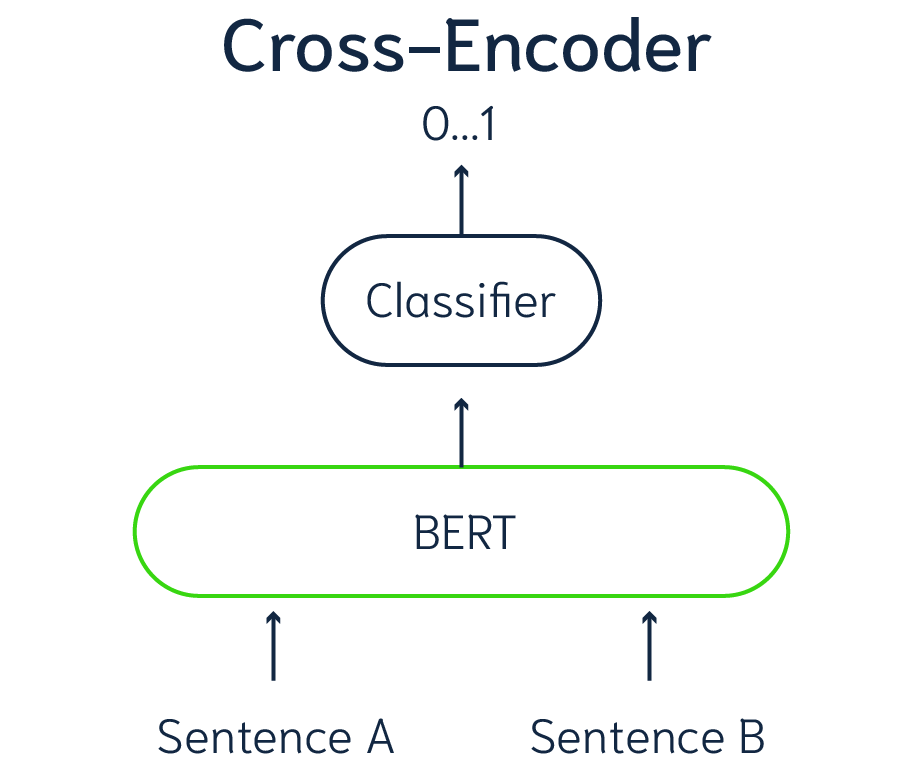
\includegraphics[width=0.5\textwidth]{Images/cross-encoder.png} % Nhớ upload ảnh và đặt đúng tên file
    \vspace{0.7cm}
    \caption{Sơ đồ kiến trúc Cross-Encoder với đầu vào ghép đôi và đầu ra phân loại}
    \label{fig:cross_encoder_arch}
% ... (Phần code chèn ảnh ở trên giữ nguyên) ...
\end{figure}

% Thêm \noindent vào đây
\noindent Quan sát Hình \ref{fig:cross_encoder_arch}, ta có thể phân tích cơ chế hoạt động qua ba giai đoạn chính:

% Thêm \noindent vào đây và dùng \vspace để tạo khoảng cách nhỏ cho thoáng
\vspace{0.2cm} 
\noindent \textbf{1. Tầng Đầu vào (Input Layer):} \\
Khác với Bi-Encoder xử lý hai nhánh độc lập, hình vẽ cho thấy Sentence A (đại diện cho truy vấn $q$) và Sentence B (đại diện cho văn bản ứng viên $d$) được đưa vào cùng một khối xử lý. Trong thực tế, hai chuỗi này được nối lại (concatenated) thành một chuỗi duy nhất, bắt đầu bằng token đặc biệt \texttt{[CLS]} và ngăn cách bởi \texttt{[SEP]}:
\begin{equation}
    Input = \texttt{[CLS]} \oplus q \oplus \texttt{[SEP]} \oplus d \oplus \texttt{[SEP]}
\end{equation}
\noindent \textbf{2. Khối xử lý trung tâm (BERT):} \\
Khối ``BERT'' trong sơ đồ đại diện cho các lớp Encoder của Transformer. Tại đây diễn ra cơ chế \textbf{Full Self-Attention} (tương tác sớm). Mỗi token trong Sentence A được phép nhìn thấy và tính toán trọng số chú ý với toàn bộ token trong Sentence B ngay từ những lớp đầu tiên. Điều này giúp mô hình nắm bắt được các sắc thái ngữ nghĩa phức tạp mà phương pháp so sánh vector độc lập thường bỏ sót.

\vspace{0.2cm}
\noindent \textbf{3. Tầng Phân loại (Classifier Head):} \\
Đầu ra của khối BERT là một chuỗi các vector ngữ cảnh, nhưng Cross-Encoder chỉ sử dụng vector tại vị trí \texttt{[CLS]} ($h_{CLS}$) để làm đại diện cho cả cặp câu. Như minh họa ở phần trên cùng của hình vẽ, vector này được đưa qua khối \textbf{Classifier} (thường là một lớp tuyến tính Linear Layer). Cuối cùng, hàm kích hoạt sẽ chuyển đổi kết quả thành một điểm số thực trong khoảng \textbf{0...1}. Giá trị này chính là xác suất phù hợp $P(y=1|q, d)$, dùng để xếp hạng lại (Reranking).

\subsubsection{So sánh hiệu năng với Bi-Encoder}


Việc lựa chọn giữa Cross-Encoder và Bi-Encoder luôn đòi hỏi sự cân nhắc kỹ lưỡng về sự đánh đổi giữa độ chính xác và hiệu suất tính toán. Để làm rõ sự khác biệt về mặt cấu trúc dẫn đến sự đánh đổi này, hãy quan sát sơ đồ so sánh dưới đây:

\begin{figure}[H]
    \centering
    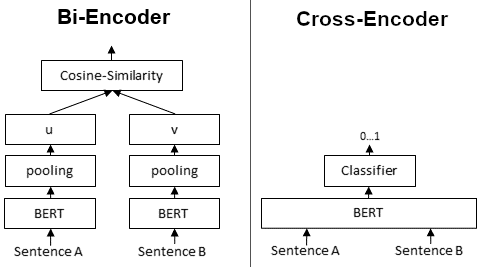
\includegraphics[width=0.8\textwidth]{Images/Bi_vs_Cross-Encoder.png} % Đảm bảo tên file ảnh đúng
    \vspace{0.5cm}
    \caption{Sơ đồ so sánh kiến trúc giữa Bi-Encoder (trái) và Cross-Encoder (phải)}
    \label{fig:bi_vs_cross}
\end{figure}


\noindent Quan sát Hình \ref{fig:bi_vs_cross}, ta thấy sự đối lập rõ rệt trong luồng xử lý dữ liệu:

\vspace{0.2cm}
\noindent \textbf{1. Về mặt Độ chính xác (Accuracy):} \\
Mô hình \textbf{Cross-Encoder} (bên phải hình vẽ) thể hiện sự vượt trội. Nhờ kiến trúc hợp nhất, cả hai câu (Sentence A và B) được đưa vào cùng một khối BERT ngay từ đầu. Điều này cho phép cơ chế Full Self-Attention hoạt động trên toàn bộ cặp câu, nắm bắt được các phụ thuộc phi tuyến tính phức tạp (non-linear dependencies). Đầu ra đi qua lớp \textit{Classifier} để trả về điểm số xác suất chính xác từ $0 \dots 1$.

Ngược lại, \textbf{Bi-Encoder} (bên trái hình vẽ) bị giới hạn bởi cấu trúc song song. Hai luồng thông tin Sentence A và Sentence B đi qua hai tháp BERT riêng biệt để tạo ra vector $u$ và $v$. Sự tương tác chỉ xảy ra ở bước cuối cùng thông qua hàm \textit{Cosine-Similarity}. Do thiếu sự tương tác sớm, Bi-Encoder thường gặp khó khăn trong các trường hợp đòi hỏi thấu hiểu ngữ nghĩa sâu hoặc khi truy vấn và văn bản có ít từ khóa chung.

\vspace{0.2cm}
\noindent \textbf{2. Về mặt Hiệu suất tính toán (Computational Efficiency):} \\
Tuy nhiên, cấu trúc tách biệt của \textbf{Bi-Encoder} lại mang đến lợi thế to lớn về tốc độ. Vì vector $v$ (đại diện cho sản phẩm) không phụ thuộc vào vector $u$ (truy vấn), chúng có thể được tính toán trước (pre-computed) và lưu trữ. Khi có truy vấn mới, hệ thống chỉ cần tính vector $u$ một lần và thực hiện tìm kiếm tương đồng (Approximate Nearest Neighbor Search) với chi phí rất thấp.

Trong khi đó, \textbf{Cross-Encoder} không thể mở rộng cho tác vụ tìm kiếm quy mô lớn. Do phải ghép nối truy vấn mới với \textit{từng} văn bản trong cơ sở dữ liệu để đưa vào mạng Transformer đồ sộ, việc áp dụng trực tiếp là bất khả thi trong thời gian thực. Vì vậy, trong thực tế, Cross-Encoder chỉ được sử dụng tối ưu trong giai đoạn Reranking trên một tập ứng viên nhỏ (ví dụ: $50-100$ items) đã được lọc sơ bộ bởi Bi-Encoder.

% ==============================================================================
% MỤC 6.2: PHƯƠNG PHÁP ĐỀ XUẤT (Tiếp nối)
% ==============================================================================

\subsection{Phương pháp đề xuất và Kiến trúc hệ thống}

Dựa trên các phân tích về hạn chế của mô hình đơn lẻ, dự án đề xuất triển khai chiến lược \textbf{Truy xuất và Xếp hạng lại (Retrieve-and-Rerank)}. Chiến lược này tận dụng sức mạnh bổ trợ của hai phương pháp mã hóa văn bản khác nhau nhằm đạt được sự cân bằng tối ưu giữa khả năng mở rộng trên dữ liệu lớn và độ chính xác trong thấu hiểu ngữ nghĩa.

\subsubsection{Quy trình Truy xuất hai giai đoạn (Two-Stage Retrieval Pipeline)}

Để giải quyết bài toán gợi ý sản phẩm với độ chính xác cao trên không gian dữ liệu lớn, hệ thống được thiết kế theo quy trình truy xuất hai giai đoạn (Retrieve-and-Rerank), hoạt động như một bộ lọc phễu từ thô đến tinh. Để hình dung rõ luồng dữ liệu và sự thay đổi về kích thước tập ứng viên qua từng bước, hãy xem xét sơ đồ quy trình dưới đây:

\begin{figure}[H]
    \centering
    % Nhớ upload file ảnh pipeline_2stage.png vào Overleaf trước
    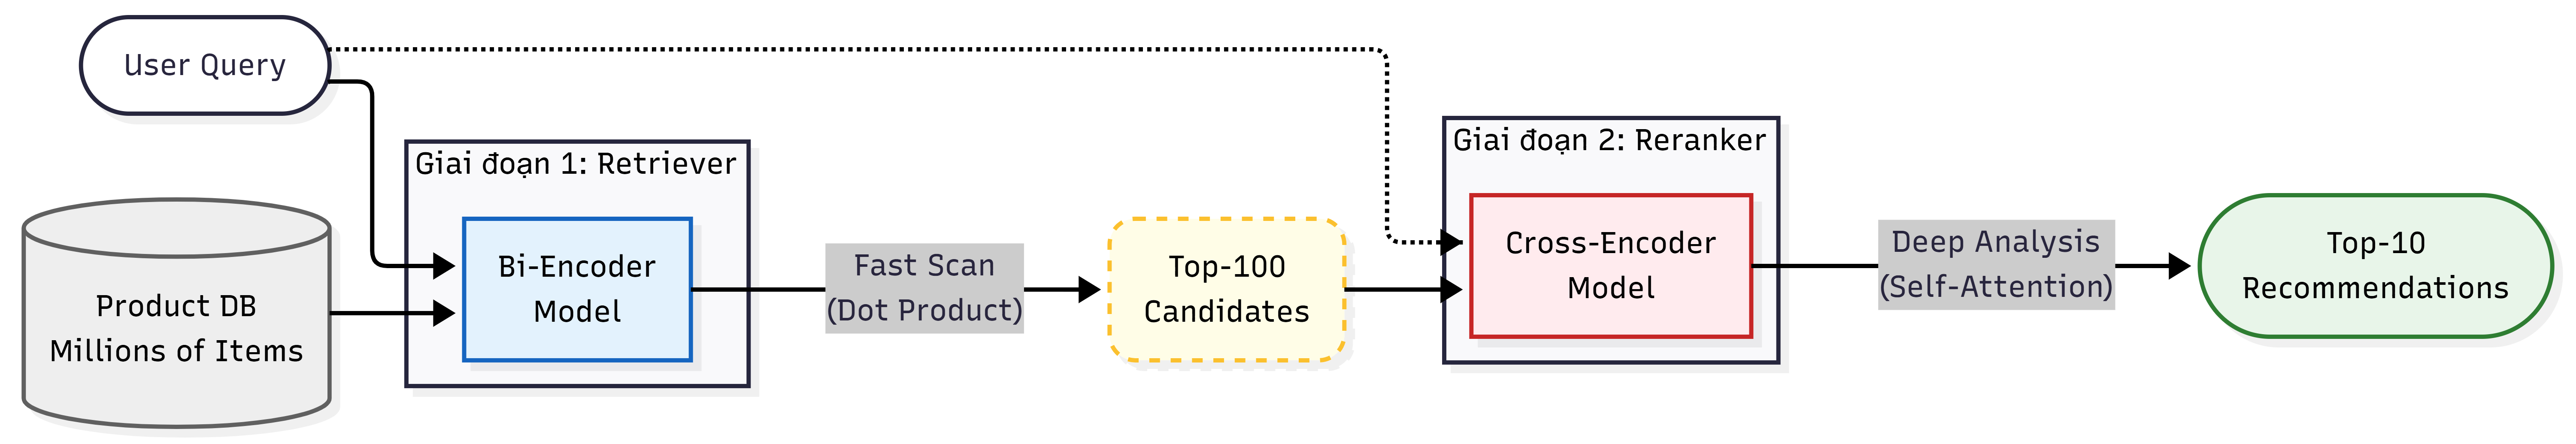
\includegraphics[width=1.0\textwidth]{Images/Two-Stage Product Retrieval-2025-12-21-060715.png}
    \vspace{0.5cm}
    \caption{Sơ đồ quy trình phễu lọc hai giai đoạn: Từ hàng triệu sản phẩm xuống Top 10}
    \label{fig:pipeline_2stage}
\end{figure}

\noindent Quan sát Hình \ref{fig:pipeline_2stage}, quy trình xử lý được chia thành hai pha riêng biệt với đặc thù trái ngược nhau về chi phí tính toán và độ chính xác:

\begin{enumerate}
    \item \textbf{Giai đoạn Sàng lọc thô (Retriever - Bi-Encoder):}
    Tại bước này (khối màu xanh dương), hệ thống quét nhanh qua toàn bộ cơ sở dữ liệu chứa hàng triệu sản phẩm. Mục tiêu là tốc độ. Đầu ra là tập hợp $K=100$ ứng viên tiềm năng nhất (khối màu vàng).
    
    \item \textbf{Giai đoạn Sàng lọc tinh (Reranker - Cross-Encoder):}
    Tập hợp 100 ứng viên được chuyển tiếp sang mô hình Cross-Encoder (khối màu đỏ). Tại đây, mô hình thực hiện phân tích ngữ cảnh sâu (Deep Analysis). Kết quả cuối cùng là Top 10 sản phẩm tối ưu nhất (khối màu xanh lá) được trả về cho người dùng.
\end{enumerate}

\noindent Trong dự án này, mô hình \texttt{cross-encoder/ms-marco-MiniLM-L6-v2} được lựa chọn làm mô hình cơ sở (base model) để tinh chỉnh (fine-tune) trên miền dữ liệu thương mại điện tử. Để mô hình có thể xử lý đồng thời thông tin người dùng và sản phẩm, dữ liệu đầu vào được cấu trúc lại thành một chuỗi token nối tiếp theo định dạng chuẩn của Transformer:
\begin{equation}
    \texttt{[CLS] Context [SEP] Candidate [SEP]}
\end{equation}
\noindent Trong cấu trúc trên, thành phần \textbf{Context} được xây dựng từ sự kết hợp giữa lịch sử tương tác và truy vấn hiện tại, giúp mô hình đối chiếu nhu cầu tìm kiếm với sở thích cá nhân. Ngay sau token ngăn cách là thành phần \textbf{Candidate}, bao gồm tiêu đề và mô tả sản phẩm, cung cấp ngữ cảnh chi tiết để mô hình đánh giá độ tương quan ngữ nghĩa.

\vspace{0.2cm} % Tạo khoảng cách nhỏ giữa Input và Output cho thoáng mắt

\noindent Quá trình tính toán kết quả cuối cùng được thực hiện tại lớp đầu ra của mạng nơ-ron. Cụ thể, vector đại diện tại vị trí \texttt{[CLS]} ($h_{CLS}$) được đưa qua một lớp tuyến tính (Linear Layer) để chiếu về một giá trị thực (logit). Giá trị này sau đó được chuyển đổi thành xác suất $P(y=1|\text{Context}, \text{Candidate})$, đại diện cho mức độ phù hợp dùng để xếp hạng sản phẩm.

% ... (Giữ nguyên phần mô tả Input/Output phía sau) ...


% ==============================================================================
% MỤC 6.2.2: LỰA CHỌN MÔ HÌNH CƠ SỞ
% ==============================================================================

\subsubsection{Lựa chọn Mô hình cơ sở: cross-encoder/ms-marco-MiniLM-L6-v2}

Để giải quyết bài toán mâu thuẫn giữa độ chính xác cao và thời gian phản hồi thấp trong hệ thống gợi ý thời gian thực, báo cáo này lựa chọn mô hình \path{cross-encoder/ms-marco-MiniLM-L6-v2}. Đây là một phiên bản mô hình ngôn ngữ được nén (compressed) từ kiến trúc BERT khổng lồ. Để hiểu rõ cơ sở khoa học của sự lựa chọn này, cần xem xét kỹ thuật nền tảng là Truyền tri thức (Knowledge Distillation) và kiến trúc đặc thù của MiniLM.

% ==============================================================================
% MỤC TỔNG QUAN VỀ KNOWLEDGE DISTILLATION (KD) - CHI TIẾT
% ==============================================================================

    % ==============================================================================
% MỤC 2.2.1 TỔNG QUAN KD (Giữ nguyên như bạn đã cung cấp)
% ==============================================================================
\paragraph{Tổng quan về Knowledge Distillation (KD)} \mbox{} \\

Trong những năm gần đây, sự bùng nổ của các Mô hình Ngôn ngữ Tiền huấn luyện (Pre-trained Language Models - PLMs) như BERT, RoBERTa hay XLNet đã tạo ra những bước đột phá trong xử lý ngôn ngữ tự nhiên. Tuy nhiên, đi kèm với hiệu suất cao là kích thước khổng lồ với hàng trăm triệu tham số. Điều này đặt ra rào cản lớn về tài nguyên tính toán và độ trễ (latency) khi triển khai trên các hệ thống thực tế hoặc thiết bị biên (edge devices).

Để giải quyết bài toán cân bằng giữa hiệu suất và tài nguyên, kỹ thuật \textbf{Truyền tri thức (Knowledge Distillation - KD)} được áp dụng như một giải pháp nén mô hình hiệu quả. Về bản chất, KD là quá trình chuyển giao khả năng khái quát hóa từ một mô hình lớn, phức tạp (Teacher) sang một mô hình nhỏ gọn hơn (Student) mà không làm giảm đáng kể độ chính xác.

Để hiểu rõ cơ chế hoạt động bên trong, hãy xem xét sơ đồ quy trình KD dưới đây:

\begin{figure}[H]
    \centering
    % Sử dụng tên file ảnh bạn đã upload
    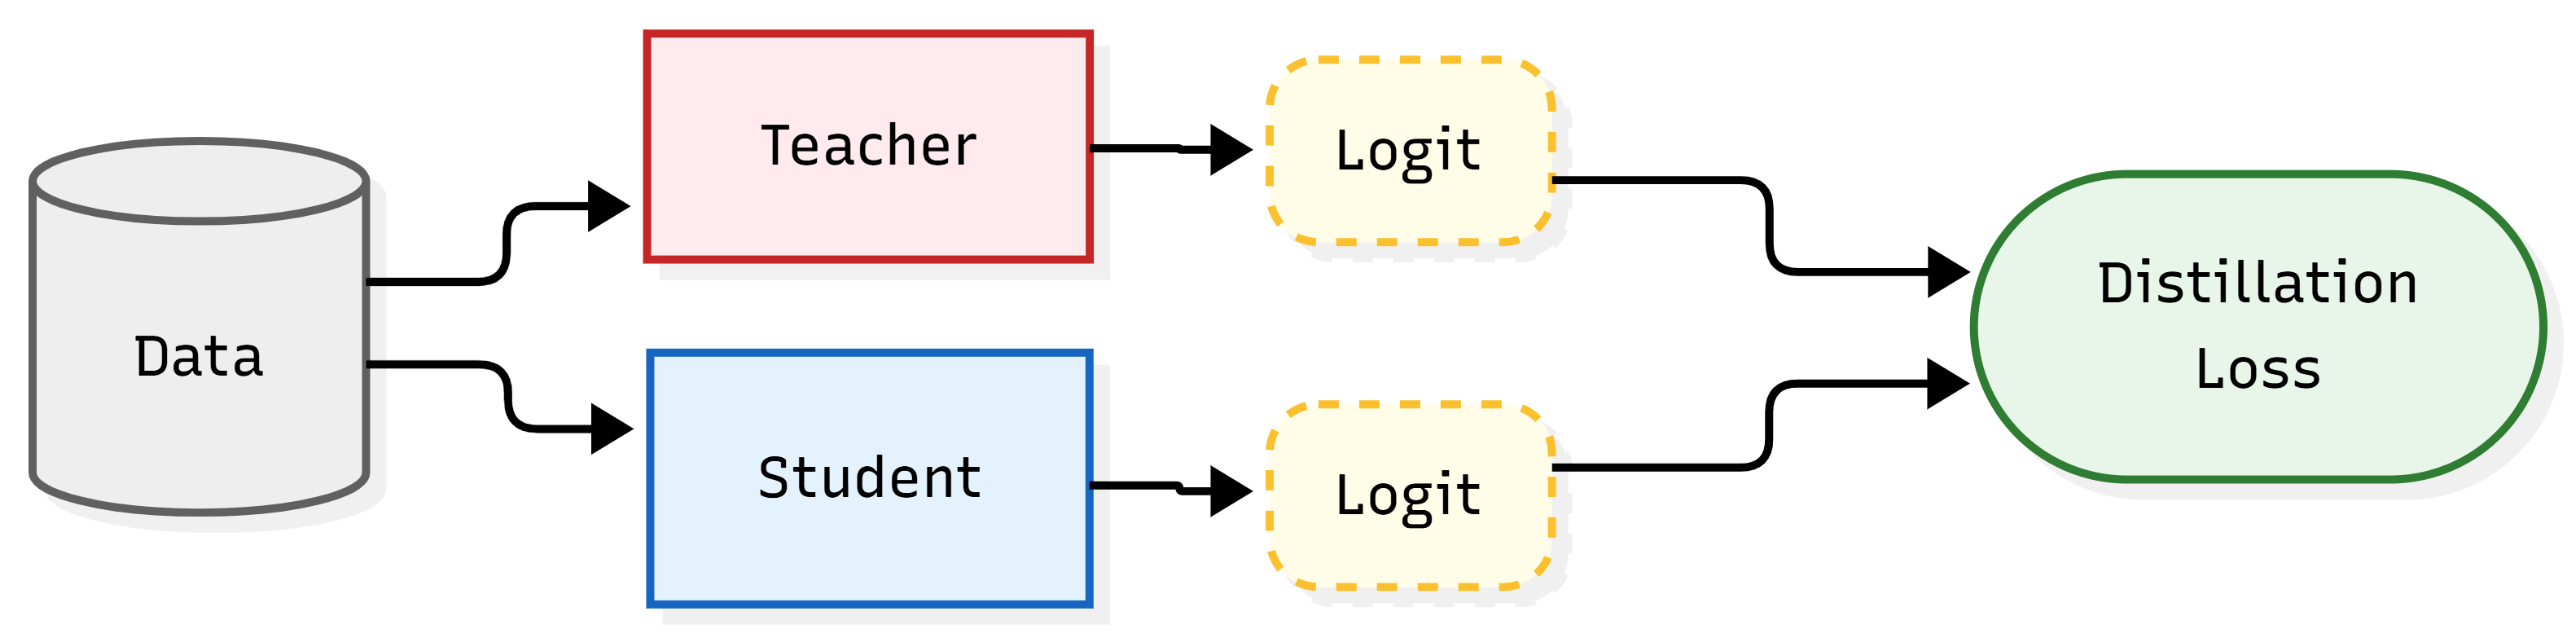
\includegraphics[width=0.9\textwidth]{Images/Untitled diagram-2025-12-21-064145.png}
    \vspace{0.5cm}
    \caption{Sơ đồ quy trình Knowledge Distillation: Mô hình Student học cách mô phỏng phân phối xác suất (Logits) của Teacher.}
    \label{fig:kd_process}
\end{figure}

\vspace{0.2cm}
\noindent Quan sát Hình \ref{fig:kd_process}, quy trình truyền tri thức bắt đầu bằng việc đưa dữ liệu đầu vào (khối \textbf{Data} màu xám) đồng thời vào hai luồng xử lý song song. Nhánh phía trên là mô hình \textbf{Teacher} (khối màu đỏ) với đặc điểm kích thước lớn và đã hội tụ, đóng vai trò nguồn tri thức chuẩn nên các trọng số thường được đóng băng để đảm bảo tính ổn định. Nhánh phía dưới là mô hình \textbf{Student} (khối màu xanh), đối tượng chính cần huấn luyện với kiến trúc được thiết kế nhỏ gọn hơn nhằm tối ưu hóa tài nguyên và tốc độ suy diễn.

\vspace{0.2cm}
\noindent Điểm cốt lõi của phương pháp này nằm ở việc khai thác thông tin từ các khối \textbf{Logit} (màu vàng). Thay vì chỉ dựa vào nhãn cứng (Hard Labels) vốn chỉ cung cấp đáp án đúng sai tuyệt đối, mô hình Student học từ phân phối xác suất đầu ra của Teacher. Các giá trị Logit này chứa đựng \textbf{Tri thức tiềm ẩn (Latent Knowledge)}—những thông tin ẩn về mối quan hệ ngữ nghĩa giữa các lớp mà nhãn cứng không thể thể hiện. Ví dụ, thông qua Logit, Teacher có thể chỉ ra rằng một đối tượng ``con chó'' có nét tương đồng về mặt đặc trưng với ``con mèo'' nhiều hơn là ``xe hơi''. Việc nắm bắt được các sắc thái tinh tế này giúp Student hình thành tư duy tổng quát hóa tốt hơn thay vì chỉ học thuộc lòng đáp án.

\vspace{0.2cm}
\noindent Cuối cùng, kết quả dự đoán của hai mô hình được đưa vào khối \textbf{Distillation Loss} (màu xanh lá) để so khớp. Đây là thành phần quan trọng nhất dùng để định hướng quá trình học, có nhiệm vụ đo lường khoảng cách giữa phân phối xác suất của Teacher và Student. Mục tiêu của quá trình huấn luyện là cực tiểu hóa sự khác biệt này, ép buộc Student phải mô phỏng lại ``cách tư duy'' của Teacher. Trong thực tế, hàm mất mát tổng thể thường là sự kết hợp có trọng số giữa hàm mất mát chưng cất (học theo Teacher) và hàm mất mát của tác vụ chính (học theo nhãn thực tế), giúp cân bằng giữa khả năng bắt chước và độ chính xác trên tập dữ liệu.

% ==============================================================================
% MỤC 2.2.2 PHÂN TÍCH MINILM (Đã chỉnh sửa phần dẫn nhập)
% ==============================================================================

% ==============================================================================
% MỤC 2.2.2 PHÂN TÍCH MINILM & LÝ DO LỰA CHỌN (ĐÃ HỢP NHẤT)
% ==============================================================================

\paragraph{Phân tích chuyên sâu về MiniLM và Ứng dụng trong Dự án} \mbox{} \\

Mặc dù phương pháp Knowledge Distillation truyền thống đã chứng minh được hiệu quả, nhưng việc áp dụng trực tiếp vào các mô hình Transformer phức tạp vẫn gặp nhiều hạn chế, đặc biệt là sự ràng buộc về kích thước chiều ẩn (Hidden Dimension) giữa Teacher và Student. Để khắc phục vấn đề này và tối ưu hóa sâu hơn vào cơ chế cốt lõi của Transformer, Wang \etal \cite{32} đã đề xuất kiến trúc \textbf{MiniLM} (Miniature Language Model). 

Khác với các phương pháp nén mô hình thông thường chỉ tập trung vào lớp đầu ra (Output Layer), MiniLM là phương pháp nén không phụ thuộc vào tác vụ (Task-Agnostic), đi sâu vào việc chưng cất thành phần quan trọng nhất tạo nên sức mạnh của Transformer: cơ chế \textbf{Self-Attention}.

\vspace{0.3cm}
\noindent \textit{1. Đặt vấn đề và Kiến thức cơ sở (Preliminary)}

Mạng Transformer được xây dựng dựa trên cơ chế Multi-Head Self-Attention. Trong một lớp Transformer, giả sử đầu vào là chuỗi vector $X$, Multi-Head Self-Attention bao gồm $H$ đầu chú ý. Tại mỗi đầu $h$, đầu vào được chiếu qua các ma trận trọng số $W_Q, W_K, W_V$ để tạo ra các vector Query ($Q_h$), Key ($K_h$) và Value ($V_h$). Công thức tính toán Standard Attention tại đầu $h$ được định nghĩa \cite{41}:

\begin{equation}
    \text{Attention}_h(Q, K, V) = \text{Softmax}\left(\frac{Q_h K_h^T}{\sqrt{d_k}}\right) V_h
\end{equation}
Trong đó $d_k$ là kích thước chiều của vector key.

\noindent \textbf{Giải thích các tham số:}
\begin{itemize}
    \item $Q_h, K_h, V_h$: Lần lượt là các ma trận Query (Truy vấn), Key (Khóa) và Value (Giá trị) tại đầu chú ý thứ $h$.
    \item $K_h^T$: Ma trận chuyển vị của $K_h$, dùng để tính tích vô hướng (độ tương đồng) với $Q_h$.
    \item $d_k$: Kích thước chiều (dimension size) của vector Key.
    \item $\sqrt{d_k}$: Hệ số tỷ lệ (scaling factor) giúp ổn định giá trị tích vô hướng trước khi đưa vào hàm Softmax.
\end{itemize}

\vspace{0.3cm}
\noindent \textit{2. Phương pháp Chưng cất Sự chú ý Sâu (Deep Self-Attention Distillation)}

MiniLM tập trung chuyển giao tri thức tại \textbf{lớp Transformer cuối cùng}, nơi chứa đựng những đặc trưng ngữ nghĩa tinh túy nhất. Quá trình này dựa trên hai thành phần cốt lõi được trình bày tại hình \ref{fig:minilm_arch}:
% --- CHÈN HÌNH ẢNH MINILM ---
\begin{figure}[H]
    \centering
    % Thay 'minilm_architecture.png' bằng tên file ảnh thực tế của bạn
    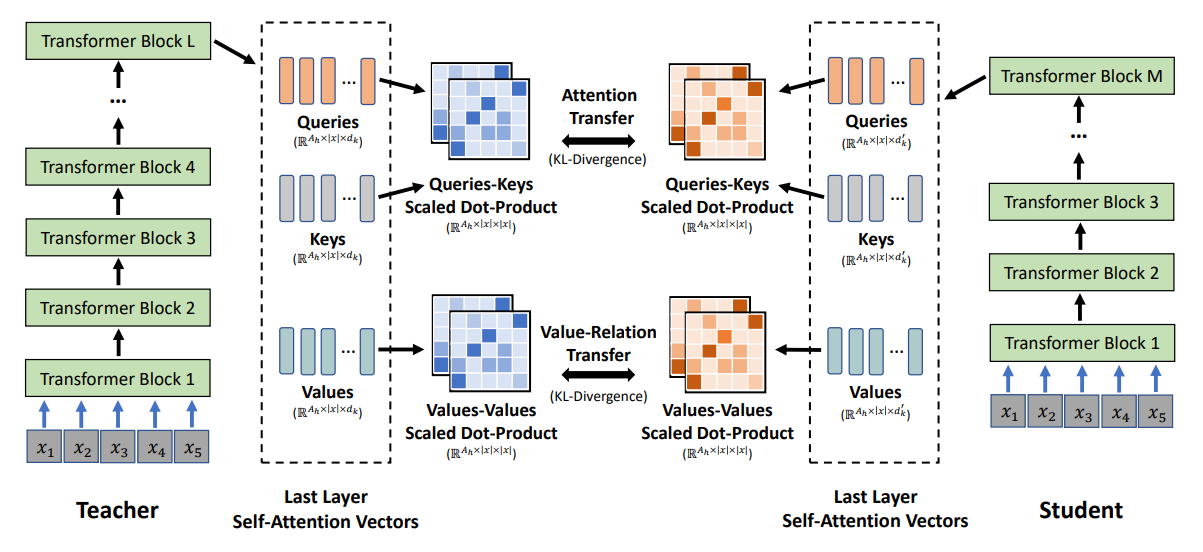
\includegraphics[width=0.9\textwidth]{Images/minilm_architecture.png} 
    \vspace{0.5cm}
    \caption{Tổng quan kiến trúc Deep Self-Attention Distillation của MiniLM.}
    \label{fig:minilm_arch}
\end{figure}


\vspace{0.2cm}

\noindent \textbf{Thành phần A: Phân phối Sự chú ý (Self-Attention Distributions).} \\
Ma trận chú ý $A_h$ biểu diễn mối quan hệ phụ thuộc giữa các từ, được tính như sau \cite{32}:

\begin{equation}
    A_h = \text{Softmax}\left(\frac{Q_h K_h^T}{\sqrt{d_k}}\right)
\end{equation}
Hàm mất mát Kullback-Leibler (KL-Divergence) được sử dụng để giảm thiểu sự khác biệt giữa Teacher ($T$) và Student ($S$):

\begin{equation}
    \mathcal{L}_{AT} = \frac{1}{H} \sum_{h=1}^{H} D_{KL}(A_h^T || A_h^S)
\end{equation}

\vspace{0.2cm}

\noindent \textbf{Thành phần B: Quan hệ Giá trị (Self-Attention Value Relations).} \\
Đây là đóng góp đột phá của MiniLM, sử dụng quan hệ giữa các vector Value ($V-V$) thay vì $Q-K$:

\begin{equation}
    VR_h = \text{Softmax}\left(\frac{V_h V_h^T}{\sqrt{d_k}}\right)
\end{equation}

Hàm mất mát tương ứng cho thành phần này là \cite{32}:


\begin{equation}
    \mathcal{L}_{VR} = \frac{1}{H} \sum_{h=1}^{H} D_{KL}(VR_h^T || VR_h^S)
\end{equation}

\noindent \textbf{Giải thích ký hiệu:}
\begin{itemize}
    \item $A_h^T, A_h^S$: Phân phối chú ý của mô hình Teacher và Student.
    \item $VR_h^T, VR_h^S$: Quan hệ giá trị của mô hình Teacher và Student.
    \item $D_{KL}$: Độ phân kỳ Kullback-Leibler, đo lường sự khác biệt giữa hai phân phối xác suất.
    \item $H$: Tổng số lượng đầu chú ý (Attention Heads).
\end{itemize}

\vspace{0.3cm}
\noindent \textit{3. Cơ sở lựa chọn phiên bản MiniLM-L6-v2 cho dự án}

\noindent Từ nền tảng lý thuyết vững chắc về cơ chế truyền tri thức kép nêu trên, phiên bản cụ thể \texttt{MiniLM-L6-v2} đã được lựa chọn để triển khai module Reranking cho hệ thống. Quyết định này dựa trên sự cân bằng tối ưu giữa hiệu quả kiến trúc, tốc độ và chất lượng. Cụ thể, với cấu hình thu nhỏ gồm 6 lớp (L6) và chiều ẩn 384, mô hình đã loại bỏ hoàn toàn sự dư thừa tham số thường thấy ở các kiến trúc lớn như BERT-Base, trong khi vẫn duy trì được khả năng suy luận ngữ nghĩa phức tạp nhờ thừa hưởng trọn vẹn Quan hệ Giá trị từ Teacher. Hơn nữa, kết quả thực nghiệm chứng minh \texttt{MiniLM-L6-v2} đạt tốc độ suy diễn (Inference) nhanh hơn gấp 2 lần so với BERT-Base. Đây là yếu tố tiên quyết đối với bài toán Reranking, giúp giữ độ trễ hệ thống ở mức thấp nhất (low latency) để đảm bảo trải nghiệm người dùng. Mặc dù kích thước giảm đi đáng kể, mô hình vẫn bảo toàn được hơn 90\% độ chính xác so với mô hình gốc trên các bảng xếp hạng chuẩn (Benchmarks), qua đó đảm bảo danh sách gợi ý cuối cùng luôn đạt độ tương quan cao nhất.


% ==============================================================================
% MỤC 6.2.2.2: ĐẶC TẢ MÔ HÌNH VÀ DỮ LIỆU
% ==============================================================================

\paragraph{Bộ dữ liệu Tiền huấn luyện: MS MARCO (Passage Ranking)} \mbox{} \\

Mô hình \texttt{cross-encoder/ms-marco-MiniLM-L6-v2} được lựa chọn làm cơ sở cho dự án nhờ vào quá trình tiền huấn luyện (pre-training) bài bản trên bộ dữ liệu \textbf{MS MARCO} (Microsoft Machine Reading Comprehension). Theo công bố khoa học của Nguyen \etal \cite{42}, đây là nền tảng quan trọng giúp mô hình học được các đặc trưng ngôn ngữ tự nhiên và logic xếp hạng thông tin từ quy mô dữ liệu lớn trước khi được tinh chỉnh cho các tác vụ cụ thể.

Điểm làm nên hiệu suất vượt trội của phiên bản mô hình này nằm ở chiến lược dữ liệu được cộng đồng \textit{Sentence-Transformers} áp dụng. Cụ thể, trong quá trình phát triển mô hình gốc, thay vì sử dụng dữ liệu thô ban đầu từ Microsoft, các tác giả đã lựa chọn phiên bản tối ưu hóa có tích hợp kỹ thuật \textbf{Hard Negatives mining}

% \footnote{\url{https://huggingface.co/datasets/sentence-transformers/msmarco-hard-negatives}}
. Kỹ thuật này tạo ra các bộ ba (Triplets) bao gồm Truy vấn, Mẫu dương và Mẫu âm, thay vì ghép cặp ngẫu nhiên. Về mặt quy mô, tập dữ liệu này bao gồm hơn 1.000.000 truy vấn thực tế từ Bing và hơn 8.800.000 đoạn văn bản, tất cả đều được gán nhãn thủ công với độ tin cậy cao.

Chính cấu trúc dữ liệu dạng Triplet này đã định hình khả năng hiểu ngữ nghĩa của mô hình trước khi được đưa vào áp dụng trong dự án. Bảng \ref{tab:msmarco_example} dưới đây minh họa mẫu dữ liệu mà mô hình đã được học, trong đó Hard Negative tuy chứa nhiều từ khóa trùng khớp (lexical overlap) nhưng sai lệch hoàn toàn về ngữ nghĩa hoặc đối tượng.


\begin{table}[H]
    \centering
    \renewcommand{\arraystretch}{1.3}
    
    \begin{tabular}{|p{0.15\textwidth}|p{0.5\textwidth}|p{0.25\textwidth}|}
        \hline
        \textbf{Thành phần} & \textbf{Nội dung văn bản} & \textbf{Phân tích ngữ nghĩa} \\
        \hline
        \textbf{Query} & \textit{``symptoms of heat exhaustion''} (Triệu chứng kiệt sức do nhiệt) & Truy vấn tìm kiếm thông tin y tế cho người. \\
        \hline
        \textbf{Positive} & \textit{``Symptoms of heat exhaustion include heavy sweating, rapid pulse...''} & Đoạn văn chứa câu trả lời chính xác, khớp ý định. \\
        \hline
        \textbf{Negative} & \textit{``Heat exhaustion is a condition whose symptoms... in dogs.''} & \textbf{Hard Negative:} Rất giống query nhưng nói về chó (dogs) thay vì người. \\
        \hline
    \end{tabular}
    \caption{Ví dụ mẫu dữ liệu Triplet trong MS MARCO với Hard Negative}
    \label{tab:msmarco_example}
\end{table}

\noindent Việc lựa chọn MS MARCO làm tiêu chuẩn vàng (Gold Standard) cho tác vụ này xuất phát từ ba đặc điểm ưu việt. Đầu tiên là tính chất thực tế (Real-world Distribution), nơi các truy vấn phản ánh đúng ngôn ngữ tự nhiên của người dùng bao gồm cả từ lóng hay lỗi chính tả, giúp mô hình bền vững hơn khi triển khai thực tế. Thứ hai là sự đa dạng về chủ đề (Topic Diversity) bao phủ từ y tế, công nghệ đến đời sống, giúp mô hình có khả năng khái quát hóa tốt. Cuối cùng và quan trọng nhất là khả năng chuyển giao (Transferability); nhờ lượng tri thức nền khổng lồ này, mô hình có thể dễ dàng thích nghi và tinh chỉnh (fine-tune) hiệu quả khi chuyển sang miền dữ liệu thương mại điện tử của Amazon.

% MỤC 6.2.2.3: ĐẶC TẢ MÔ HÌNH CROSS-ENCODER (Đưa xuống sau)
% ==============================================================================
\paragraph{Đặc tả Mô hình Cross-Encoder: cross-encoder/ms-marco-MiniLM-L6-v2} \mbox{} \\

Sau khi xác lập kiến trúc nền tảng là MiniLM và bộ dữ liệu nguồn là MS MARCO, dự án lựa chọn phiên bản cụ thể \texttt{cross-encoder/ms-marco-MiniLM-L6-v2}\footnote{Link mô hình: \url{https://huggingface.co/cross-encoder/ms-marco-MiniLM-L6-v2}} làm điểm khởi đầu (checkpoint) cho quá trình huấn luyện. Đây không phải là một mô hình được khởi tạo ngẫu nhiên, mà là kết quả của một \textbf{quy trình huấn luyện kế thừa (Multi-stage Training Pipeline)} được thực hiện bài bản qua nhiều giai đoạn.

\vspace{0.2cm}
\noindent \textbf{1. Nguồn gốc và Quy trình hình thành} \\
Quá trình phát triển mô hình (hình \ref{fig:model_creation}) bắt đầu từ kiến trúc \textit{MiniLM gốc} của Microsoft, được nén từ BERT để học các biểu diễn ngôn ngữ chung (General Language Understanding). Ở giai đoạn thích nghi (Adaptation), mô hình được chuyển đổi sang định dạng tương thích với thư viện \textit{Sentence-Transformers} (phiên bản \texttt{nreimers/MiniLM-L6-H384-uncased}). Tuy nhiên, bước ngoặt quyết định nằm ở giai đoạn tinh chỉnh (Fine-tuning), nơi mô hình được huấn luyện chuyên sâu trên tập dữ liệu \textbf{MS MARCO Passage Ranking}. Mục tiêu của giai đoạn này là trang bị cho mô hình kỹ năng xếp hạng và phân biệt đoạn văn phù hợp với câu hỏi, chuyển hóa từ một mô hình ngôn ngữ chung thành một Cross-Encoder chuyên dụng. Cuối cùng, để tối ưu hóa cho môi trường thực tế, các trọng số đã được Quantized nhằm giảm kích thước và tăng tốc độ suy diễn.

\begin{figure}[H]
    \centering
    % Đảm bảo đường dẫn ảnh đúng với thư mục trong Overleaf của bạn
    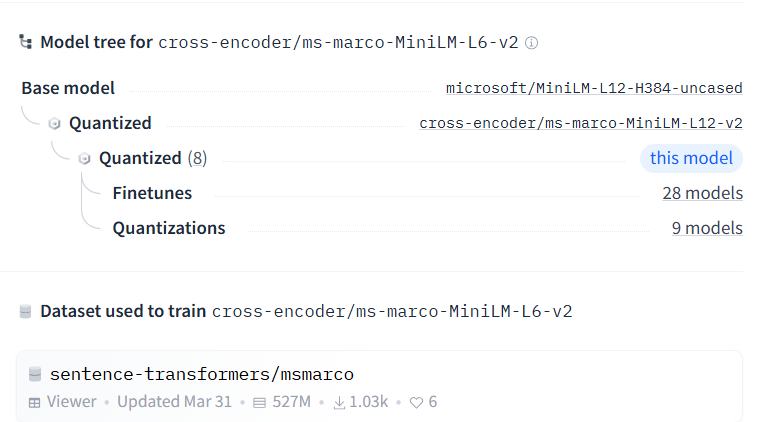
\includegraphics[width=0.9\textwidth]{Images/model_lineage.png}
    \vspace{1cm}
    \caption{Quy trình phát triển mô hình: Từ kiến trúc MiniLM gốc, qua bước tinh chỉnh (Fine-tuning) trên dữ liệu MS MARCO để tạo thành Cross-Encoder hoàn chỉnh.}
    \label{fig:model_creation}
\end{figure}

\noindent \textbf{2. Thông số kỹ thuật và Kiến trúc mạng} \\
Về mặt đặc tả kỹ thuật, mô hình sở hữu cấu trúc gọn nhẹ với \textbf{6 lớp Transformer (Layers)}, chiều ẩn (Hidden size) 384 và 12 Attention Head, tổng hợp thành khoảng \textbf{22.7 triệu tham số}. Khác với các mô hình BERT tiêu chuẩn (thường có hơn 110 triệu tham số), kích thước này cho phép triển khai hiệu quả trên các hệ thống có tài nguyên hạn chế.

Dữ liệu đầu vào của mô hình được xử lý theo cơ chế nối tiếp cặp văn bản: \texttt{[CLS] Query [SEP] Passage [SEP]}, với tổng độ dài tối đa cho phép là \textbf{512 tokens}. Tại đầu ra, một lớp tuyến tính (Linear Layer) được gắn trực tiếp trên token \texttt{[CLS]} để thực hiện nhiệm vụ hồi quy, dự đoán điểm số logit $s \in (-\infty, +\infty)$ biểu thị mức độ phù hợp ngữ nghĩa giữa truy vấn và văn bản.

% ==============================================================================
% MỤC 6.3.1: CHUẨN BỊ DỮ LIỆU HUẤN LUYỆN
% ==============================================================================

% ==============================================================================
% MỤC 6.3: CHIẾN LƯỢC TINH CHỈNH (FINE-TUNING STRATEGY)
% ==============================================================================

\subsubsection{Chiến lược Tinh chỉnh mô hình (Fine-tuning Strategy)}

Mặc dù mô hình nền tảng \texttt{cross-encoder/ms-marco-MiniLM-L6-v2} đã sở hữu năng lực xếp hạng văn bản ấn tượng nhờ quá trình tiền huấn luyện trên dữ liệu MS MARCO, việc áp dụng trực tiếp mô hình này vào bài toán thương mại điện tử gặp phải thách thức lớn về sự \textbf{sai lệch miền dữ liệu (Domain Shift)}.

Dữ liệu MS MARCO chủ yếu là các câu hỏi tìm kiếm thông tin chung (General Web Search), trong khi truy vấn trên Amazon mang tính chất giao dịch (Transactional Queries), chứa đựng nhiều mã định danh sản phẩm (ASIN), tên thương hiệu cụ thể và các từ khóa đặc thù ngành hàng (như ``OLED'', ``noise-cancelling''). Hơn nữa, hành vi tìm kiếm của người dùng thương mại điện tử đòi hỏi độ chính xác cực cao.

Do đó, dự án đề xuất chiến lược tinh chỉnh (Fine-tuning) dựa trên nguyên lý \textbf{Chuyển giao tri thức (Transfer Learning)}. Mục tiêu là chuyển đổi một mô hình xếp hạng văn bản phổ thông thành một chuyên gia xếp hạng sản phẩm. Quá trình này được thực hiện thông qua việc huấn luyện giám sát trên hai nguồn dữ liệu bổ trợ nhau: dữ liệu hành vi thực tế (ESCI) và dữ liệu tổng hợp từ AI \cite{34}.

% ------------------------------------------------------------------------------
% MỤC 6.3.1: CHUẨN BỊ DỮ LIỆU
% ------------------------------------------------------------------------------

\paragraph{Chuẩn bị dữ liệu huấn luyện} \mbox{} \\

Chất lượng của mô hình Cross-Encoder phụ thuộc tiên quyết vào chất lượng của các cặp dữ liệu \texttt{(Query, Product, Label)}. Để đạt được sự cân bằng giữa độ chính xác từ khóa và khả năng thấu hiểu ngôn ngữ tự nhiên, hệ thống dữ liệu huấn luyện được xây dựng từ hai nguồn chính.
\vspace{0.5cm}

% ==============================================================================
% MỤC 1: BỘ DỮ LIỆU ESCI
% ==============================================================================

\noindent \textbf{1. Bộ dữ liệu ESCI (Amazon Shopping Queries)} \\
Nguồn dữ liệu cốt lõi được sử dụng để tinh chỉnh mô hình là bộ dữ liệu \textbf{ESCI (Shopping Queries Dataset)}. Đây là tập dữ liệu quy mô lớn được công bố bởi nhóm nghiên cứu Amazon Science, được cộng đồng học thuật công nhận là tiêu chuẩn vàng để đánh giá các thuật toán tìm kiếm sản phẩm \cite{33}.

Điểm đặc biệt của bộ dữ liệu này nằm ở hệ thống nhãn đa cấp độ, được viết tắt là \textbf{ESCI}, mô tả chính xác sắc thái ngữ nghĩa giữa truy vấn của người dùng và sản phẩm trả về. Cụ thể, bốn mức độ tương quan được định nghĩa như sau:

\begin{itemize}
    \item \textbf{Exact (E - Khớp hoàn toàn):} Sản phẩm đáp ứng chính xác nhu cầu của người dùng về mọi mặt như chức năng, thương hiệu và thông số kỹ thuật (Ví dụ: Tìm ``iPhone 12'' và kết quả là điện thoại iPhone 12).
    \item \textbf{Substitute (S - Thay thế):} Sản phẩm có chức năng tương đương nhưng khác biệt về một số đặc tính quan trọng như thương hiệu, màu sắc hoặc mẫu mã, mà người dùng có thể cân nhắc nếu sản phẩm chính hết hàng (Ví dụ: Tìm ``giày chạy bộ Nike'' nhưng kết quả là ``giày Adidas'').
    \item \textbf{Complement (C - Bổ trợ):} Sản phẩm không thỏa mãn trực tiếp truy vấn nhưng thường được mua kèm hoặc hỗ trợ cho sản phẩm chính (Ví dụ: Tìm ``iPhone 12'' nhưng kết quả là ``Ốp lưng'' hoặc ``Dây sạc'').
    \item \textbf{Irrelevant (I - Không liên quan):} Sản phẩm hoàn toàn không liên quan đến truy vấn.
\end{itemize}

\begin{table}[H]
    \centering
    \caption{Ví dụ minh họa và chiến lược gán nhãn nhị phân cho ESCI}
    
    \small 
    \renewcommand{\arraystretch}{1.3} % Tăng khoảng cách dòng cho thoáng
    % Tổng độ rộng các cột: 0.18 + 0.32 + 0.12 + 0.28 = 0.90\textwidth (Vừa vặn)
    \begin{tabular}{|p{0.18\textwidth}|p{0.32\textwidth}|p{0.12\textwidth}|p{0.28\textwidth}|}
        \hline
        \centering \textbf{Truy vấn} & \centering \textbf{Sản phẩm} & \centering \textbf{Nhãn gốc} & \textbf{Chiến lược Cross-Encoder} \\
        \hline
        iphone 12 case & OtterBox Commuter Case for iPhone 12 & \textbf{Exact} & \textbf{Positive (1):} Khớp hoàn toàn ý định. \\
        \hline
        iphone 12 case & iPhone 12 64GB Black (Unlocked) & \textbf{Irrelevant} & \textbf{Negative (0):} Sai loại sản phẩm. \\
        \hline
        nike running shoes & Adidas Ultraboost 21 Men's Shoe & \textbf{Substitute} & \textbf{Hard Negative (0):} Sai thương hiệu dù cùng chức năng. \\
        \hline
        camera canon & SD Card 64GB & \textbf{Complement} & \textbf{Hard Negative (0):} Sản phẩm đi kèm, không phải sản phẩm chính. \\
        \hline
    \end{tabular}
    \caption{Ví dụ minh họa và chiến lược gán nhãn nhị phân cho ESCI}
    \label{tab:esci_examples}
\end{table}

\noindent Vì Cross-Encoder trong dự án được thiết kế cho bài toán phân loại nhị phân (Binary Classification), hệ thống nhãn ESCI cần được quy hoạch lại một cách chiến lược. Theo đó, chỉ duy nhất nhãn \textbf{Exact} được coi là mẫu Dương (Label = 1). Tất cả các nhãn còn lại bao gồm Substitute, Complement và Irrelevant đều được gán là mẫu Âm (Label = 0). 

Chiến lược gán nhãn này đóng vai trò quan trọng trong việc tạo ra \textbf{(Hard Negatives)}. Đặc biệt, việc ép nhãn Substitute và Complement về 0 giúp mô hình học được sự phân biệt tinh tế: dù ``Adidas'' và ``Nike'' có sự tương đồng lớn về ngữ nghĩa vector (cùng là giày thể thao), nhưng trong ngữ cảnh tìm kiếm cụ thể, sự sai lệch về thương hiệu là không thể chấp nhận. Điều này giúp Cross-Encoder nắm bắt chặt chẽ các thực thể thương mại và ý định người dùng tốt hơn so với các phương pháp so khớp từ khóa thông thường.

\vspace{0.5cm} % Tạo khoảng cách giữa 2 mục

% --- 6.3.1.2 BLAIR DATASET ---

% --- 6.3.1.2 BLAIR DATASET ---

\noindent \textbf{2. Bộ dữ liệu Tổng hợp từ AI (Phương pháp BLAIR)} \\
Một hạn chế lớn của bộ dữ liệu ESCI là các truy vấn thường ngắn, thiên về từ khóa và thiếu cấu trúc ngữ pháp hoàn chỉnh. Trong khi đó, xu hướng người dùng thực tế ngày càng sử dụng các câu hỏi dài, mô tả nhu cầu phức tạp hoặc tìm kiếm bằng ngôn ngữ tự nhiên. Để lấp đầy khoảng trống này, phương pháp tạo dữ liệu tổng hợp dựa trên kỹ thuật \textbf{BLAIR} (Bridging Language and Items for Retrieval) được áp dụng để sinh ra các mẫu huấn luyện giàu ngữ nghĩa của Hou \etal \cite{34}.

\textbf{Quy trình sinh dữ liệu (Reverse Engineering):} \\
Để giải quyết vấn đề khan hiếm dữ liệu truy vấn phức tạp, quy trình Kỹ thuật đảo ngược được thực hiện bằng cách sử dụng Mô hình Ngôn ngữ Lớn (LLM) như GPT-4 hoặc Gemini. Quy trình này dựa trên giả định rằng nội dung đánh giá chi tiết chính là sự phản ánh nhu cầu tìm kiếm của người dùng nhưng ở thì quá khứ.

Các bước thực hiện cụ thể như sau:
\begin{enumerate}
    \item \textbf{Lựa chọn nguồn dữ liệu:} Các bài đánh giá từ tập dữ liệu Amazon Reviews 2023 được chọn làm đầu vào. Để đảm bảo chất lượng, dữ liệu được lọc theo tiêu chuẩn nghiêm ngặt: chỉ chọn các đánh giá \textbf{5 sao} (thể hiện sự hài lòng tuyệt đối với sản phẩm) và có độ dài tối thiểu \textbf{100 ký tự} (đảm bảo cung cấp đủ ngữ cảnh và thông tin chi tiết).
    \item \textbf{Prompting (Tạo câu lệnh):} LLM được yêu cầu đóng vai một người mua hàng tiềm năng, đọc nội dung review và viết lại thành một câu truy vấn tìm kiếm (Search Query) dưới góc nhìn thứ nhất, sao cho sản phẩm đó là câu trả lời phù hợp nhất.
    \item \textbf{Kết quả đầu ra:} Tạo thành các cặp dữ liệu \texttt{(Synthetic Query, Product)} với nhãn là Positive (1).
\end{enumerate}

\begin{table}[H]
    \centering
    
    \label{tab:blair_examples}
    \small
    \begin{tabular}{|p{0.35\textwidth}|p{0.35\textwidth}|p{0.2\textwidth}|}
        \hline
        \textbf{Review Gốc (Input)} & \textbf{Synthetic Query (Output bởi AI)} & \textbf{Sản phẩm} \\
        \hline
        ``Tôi thường xuyên phải bay đường dài và chiếc tai nghe này thực sự cứu cánh. Chức năng chống ồn chặn hoàn toàn tiếng động cơ máy bay. Pin dùng liên tục 30 tiếng vẫn chưa hết...'' & ``Tôi cần tìm một chiếc tai nghe chụp tai có khả năng chống ồn chủ động tốt nhất để đi máy bay và làm việc tập trung, yêu cầu thời lượng pin trâu.'' & Sony Headphones \\
        \hline
        ``Giày rất êm, phần đệm lót hỗ trợ cực tốt cho người bị bàn chân bẹt như tôi. Tôi đã chạy marathon mà không hề bị đau gan bàn chân.'' & ``Giày chạy bộ chuyên dụng tốt nhất giúp giảm đau và hỗ trợ chỉnh hình cho người có vòm bàn chân thấp hoặc bàn chân bẹt.'' & Adidas Shoes\\
        \hline
    \end{tabular}
    \caption{Ví dụ minh họa quy trình sinh dữ liệu tổng hợp từ Review}
\end{table}

\textbf{Tác dụng của bộ dữ liệu:} \\
Phương pháp này giúp tạo ra hàng nghìn cặp dữ liệu huấn luyện chất lượng cao. Các truy vấn tổng hợp này mang ngữ nghĩa phong phú hơn rất nhiều so với từ khóa đơn thuần, giúp mô hình Cross-Encoder học được cách xử lý các câu hỏi dài, nắm bắt được nhu cầu ẩn (latent needs) và ngữ cảnh sử dụng cụ thể của người dùng.

% ==============================================================================
% MỤC 6.3.2: KỸ THUẬT KHAI THÁC MẪU ÂM (HARD NEGATIVE MINING)
% ==============================================================================

\paragraph{Kỹ thuật khai thác mẫu âm (Hard Negative Mining)} \mbox{} \\

Trong bài toán xếp hạng và truy vấn thông tin, việc lựa chọn dữ liệu huấn luyện đóng vai trò quyết định đến độ chính xác của mô hình. Trong khi các mẫu dương (Positive samples) thường được xác định rõ ràng dựa trên nhãn dữ liệu (ví dụ: sản phẩm người dùng đã mua hoặc đánh giá 5 sao), việc lựa chọn mẫu âm (Negative samples) lại phức tạp hơn nhiều. Dự án áp dụng kỹ thuật \textbf{Khai thác mẫu âm khó (Hard Negative Mining)} để tối ưu hóa quá trình huấn luyện Cross-Encoder.

\vspace{0.3cm}
\noindent \textbf{Cơ sở lý thuyết và Sự cần thiết} \\
Thông thường, các phương pháp huấn luyện cơ bản sử dụng \textit{Mẫu âm ngẫu nhiên (Random Negatives)} -- tức là ghép một truy vấn bất kỳ với một sản phẩm được chọn ngẫu nhiên từ kho hàng. Tuy nhiên, phương pháp này bộc lộ hạn chế lớn khi áp dụng cho Cross-Encoder:
\begin{itemize}
    \item \textbf{Vấn đề hội tụ chậm (Inefficient Learning):} Trong không gian vector khổng lồ của hàng triệu sản phẩm, đại đa số các sản phẩm ngẫu nhiên là Dễ phân biệt (Easy Negatives). Ví dụ, với truy vấn \textit{``Laptop gaming''}, một mẫu âm ngẫu nhiên như \textit{``Nồi cơm điện''} hoàn toàn khác biệt về mặt ngữ nghĩa. Mô hình sẽ rất nhanh chóng đẩy xác suất của cặp này về 0, dẫn đến giá trị hàm mất mát (Loss) xấp xỉ 0 và triệt tiêu đạo hàm (vanishing gradients). Kết quả là mô hình ngừng học hỏi dù chưa thực sự hiểu sâu về đặc điểm sản phẩm.
    \item \textbf{Nhu cầu về khả năng phân biệt tinh tế:} Các nghiên cứu về Truy vấn thông tin mật độ cao (Dense Retrieval) của Karpukhin \etal \cite{35} đã chỉ ra rằng hiệu suất xếp hạng được cải thiện đáng kể khi mô hình được tiếp xúc với các mẫu nằm sát đường ranh giới quyết định (Decision Boundary). Đây là những mẫu sai nhưng nhìn có vẻ đúng.
\end{itemize}
Do đó, Hard Negative Mining là bắt buộc để ép Cross-Encoder phải học các đặc trưng chi tiết thay vì chỉ dựa vào các từ khóa bề mặt.

\vspace{0.3cm}
\noindent \textbf{Quy trình Khai thác mẫu khó} \\
Quy trình tạo mẫu âm khó được thực hiện trong giai đoạn tiền xử lý dữ liệu (Offline Pre-processing), tận dụng sức mạnh của mô hình Bi-Encoder để sàng lọc ứng viên. Các bước thực hiện cụ thể như sau:

\begin{enumerate}
    \item \textbf{Truy xuất ứng viên (Candidate Retrieval):} Sử dụng một mô hình Bi-Encoder (dạng kiến trúc Sentence-BERT gọn nhẹ) để mã hóa toàn bộ truy vấn trong tập huấn luyện và toàn bộ sản phẩm trong kho hàng thành các vector. Với mỗi truy vấn $q$, hệ thống thực hiện tìm kiếm Top-K (với $K=50$) sản phẩm có độ tương đồng vector cao nhất.
    \item \textbf{Lọc bỏ nhãn dương (Filtering Positives):} Trong danh sách 50 sản phẩm được Bi-Encoder gợi ý, hệ thống loại bỏ các sản phẩm trùng với nhãn dương (Ground Truth -- sản phẩm thực tế người dùng đã chọn) dựa trên ID sản phẩm.
    \item \textbf{Xác định Mẫu âm khó (Hard Negatives Identification):} Các sản phẩm còn lại trong Top-K chính là \textit{Hard Negatives}. Đặc điểm của chúng là có điểm tương đồng vector rất cao với truy vấn (do đó Bi-Encoder mới xếp vào top đầu), nhưng về mặt chức năng hoặc ý định người dùng thì chúng là kết quả sai. Các mẫu này thường chia sẻ nhiều từ khóa quan trọng với truy vấn hoặc thuộc cùng một danh mục sản phẩm, dễ gây nhầm lẫn cho các mô hình đơn giản.
\end{enumerate}

\vspace{0.3cm}
\noindent \textbf{Ví dụ minh họa thực tế} \\
Để làm rõ hiệu quả của phương pháp, hãy xem xét ví dụ với truy vấn \textbf{``iPhone 12''}:
\begin{itemize}
    \item \textbf{Random Negative:} \textit{``Giày Adidas''} $\rightarrow$ Quá dễ, Cross-Encoder không học được gì.
    \item \textbf{Hard Negative (Sinh ra từ Bi-Encoder):} \textit{``Ốp lưng iPhone 12 Pro Max''}.
\end{itemize}

Sản phẩm ốp lưng này chứa toàn bộ các từ khóa trong truy vấn (``iPhone'', ``12'') và vector ngữ nghĩa rất gần với điện thoại. Bi-Encoder thường không phân biệt tốt mối quan hệ giữa ``vật thể'' (điện thoại) và ``phụ kiện'' (ốp lưng). Khi đưa cặp \texttt{(``iPhone 12'', ``Ốp lưng iPhone 12 Pro Max'')} vào huấn luyện với nhãn 0, Cross-Encoder buộc phải chú ý đến từ khóa ``Ốp lưng'' (Case) để phạt nặng điểm số xuống thấp. Nhờ đó, mô hình học được sự phân biệt ngữ nghĩa sâu sắc mà Bi-Encoder đã bỏ sót.

\paragraph{Phương pháp huấn luyện} \mbox{} \\
% ==============================================================================
% MỤC 6.3.3: PHƯƠNG PHÁP HUẤN LUYỆN
% ==============================================================================

Để đảm bảo mô hình Cross-Encoder hội tụ ổn định và đạt hiệu suất tối ưu trên miền dữ liệu thương mại điện tử, quá trình huấn luyện được thiết lập dựa trên các kỹ thuật tiêu chuẩn của kiến trúc Transformer hiện đại. Các thành phần chính của quy trình huấn luyện bao gồm:

\vspace{0.3cm}
\noindent \textbf{Hàm mất mát (Loss Function):} \\
Dự án sử dụng hàm \textbf{Binary Cross-Entropy with Logits (BCEWithLogitsLoss)}. Vì bản chất của Cross-Encoder trong hệ thống này là giải quyết bài toán phân loại nhị phân (xác định một cặp \texttt{Query-Product} là Phù hợp hoặc Không phù hợp), mô hình sẽ xuất ra một giá trị thực (logits) thể hiện mức độ tương đồng. Hàm \texttt{BCEWithLogitsLoss} tích hợp lớp Sigmoid và hàm Cross-Entropy vào một bước tính toán duy nhất, giúp đảm bảo tính ổn định số học (numerical stability). Mục tiêu là tối thiểu hóa sai số giữa xác suất dự đoán và nhãn thực tế (1 cho Exact match và 0 cho các trường hợp còn lại).

\vspace{0.3cm}
\noindent \textbf{Trình tối ưu hóa (Optimizer):} \\
Chúng tôi lựa chọn \textbf{AdamW} (Adam with Weight Decay) làm thuật toán tối ưu hóa. Đây là tiêu chuẩn vàng cho việc huấn luyện các mô hình ngôn ngữ lớn như BERT hay RoBERTa. Khác với Adam truyền thống, AdamW tách biệt việc suy giảm trọng số (Weight Decay) khỏi việc tính toán gradient, giúp mô hình tổng quát hóa tốt hơn và hạn chế hiện tượng quá khớp (overfitting) trên tập dữ liệu huấn luyện.

\vspace{0.3cm}
\noindent \textbf{Cơ chế lập lịch tốc độ học (Learning Rate Scheduler):} \\
Việc huấn luyện Transformer rất nhạy cảm với tốc độ học. Nếu tốc độ học quá lớn ngay từ đầu, mô hình dễ bị mất ổn định (gradient explosion). Do đó, chiến lược \textbf{Linear Warmup} được áp dụng. Cụ thể, trong 10\% tổng số bước huấn luyện đầu tiên (warmup steps), tốc độ học sẽ tăng tuyến tính từ 0 lên mức tối đa (ví dụ $2e^{-5}$). Giai đoạn làm nóng này giúp các trọng số của mô hình di chuyển về vùng không gian tham số ổn định trước khi bắt đầu quá trình tối ưu hóa chính thức. Sau đó, tốc độ học giảm dần tuyến tính về 0 để giúp mô hình hội tụ tốt hơn.

\vspace{0.3cm}
\noindent \textbf{Chỉ số đánh giá (Evaluation Metrics):} \\
Do đặc thù của bài toán Reranking là sắp xếp thứ tự ưu tiên, việc sử dụng độ chính xác (Accuracy) đơn thuần là không phản ánh đúng trải nghiệm người dùng. Thay vào đó, hiệu năng mô hình được đo lường bằng các chỉ số xếp hạng chuyên dụng trên tập Validation:
\begin{itemize}
    \item \textbf{NDCG@10 (Normalized Discounted Cumulative Gain):} Đây là chỉ số quan trọng nhất, đo lường chất lượng xếp hạng có trọng số. NDCG đánh giá cao việc đưa các kết quả đúng lên các vị trí đầu tiên (top 1, top 2) hơn là các vị trí thấp hơn trong danh sách top 10.
    \item \textbf{MRR@10 (Mean Reciprocal Rank):} Đo lường nghịch đảo thứ hạng của kết quả đúng đầu tiên tìm được. Chỉ số này cho biết trung bình người dùng phải lướt xuống bao xa để thấy kết quả mong muốn đầu tiên.
\end{itemize}

\section{Kế hoạch thực hiện đề tài}
\begin{table}[H]
    \centering
    \caption{Kế hoạch thực hiện đề tài (15 Tuần)}
    \label{tab:project-timeline}
    \renewcommand{\arraystretch}{1.3}
    \begin{tabularx}{1.0\linewidth}{lX}
    \toprule
    \textbf{Tuần (Thời gian)} & \textbf{Nội dung thực hiện} \\
    \midrule
    Tuần 01 (12/01 -- 18/01) & Thiết lập môi trường và quy hoạch nhãn dữ liệu ESCI (Exact=1, còn lại=0). \\
    Tuần 02 (19/01 -- 25/01) & Khai thác Hard Negatives từ Demo Bi-Encoder cũ (Lọc các ca dự đoán sai). \\
    Tuần 03 (26/01 -- 01/02) & Sinh dữ liệu giả lập BLAIR (Dùng LLM tạo Query từ Review 5 sao). \\
    Tuần 04 (02/02 -- 08/02) & Tổng hợp dữ liệu (ESCI + Hard Neg + BLAIR) và phân chia tập Train/Val/Test. \\
    Tuần 05 (09/02 -- 15/02) & Huấn luyện Baseline (Fine-tune Cross-Encoder chỉ trên tập ESCI gốc). \\
    Tuần 06 (16/02 -- 22/02) & Huấn luyện Nâng cao trên toàn bộ dữ liệu, giám sát hàm Loss để tránh Overfitting. \\
    Tuần 07 (23/02 -- 01/03) & Đánh giá mô hình (NDCG@10, MRR@10) trên tập Test và so sánh với Baseline. \\
    Tuần 08 (02/03 -- 08/03) & Phân tích lỗi (Error Analysis) và tinh chỉnh Hyperparameters để tối ưu kết quả. \\
    Tuần 09 (09/03 -- 15/03) & Xây dựng API Reranking và tích hợp vào hệ thống (Pipeline: Retrieve $\to$ Rerank). \\
    Tuần 10 (16/03 -- 22/03) & Lượng tử hóa mô hình (Quantization FP32 $\to$ INT8) để tối ưu thời gian phản hồi. \\
    Tuần 11 (23/03 -- 29/03) & Kiểm tra chịu tải (Stress Test) và đánh giá độ trễ tổng thể của hệ thống. \\
    Tuần 12 (30/03 -- 05/04) & Cập nhật Frontend Demo, thu thập số liệu và chụp ảnh minh họa cho báo cáo. \\
    Tuần 13 (06/04 -- 12/04) & Viết báo cáo: Cơ sở lý thuyết, Dữ liệu (BLAIR, Hard Negs), Kiến trúc hệ thống. \\
    Tuần 14 (13/04 -- 19/04) & Viết báo cáo: Kết quả thực nghiệm, Kết luận. Rà soát lỗi và chỉnh sửa. \\
    Tuần 15 (20/04 -- 26/04) & Thiết kế Slide thuyết trình, quay Video Demo và hoàn tất hồ sơ bảo vệ. \\
    \bottomrule
    \end{tabularx}
\end{table}